\chapter{Exercise 04}
\extitle{Regularized Linear Gradient}
%******************************************************************************%
%                                                                              %
%                                 Interlude                                    %
%                         for Machine Learning module                          %
%                                                                              %
%******************************************************************************%

% =============================================== %
\section*{Interlude - Regularized Gradient}
% =============================================== %
\begin{figure}[!h]
    \centering
    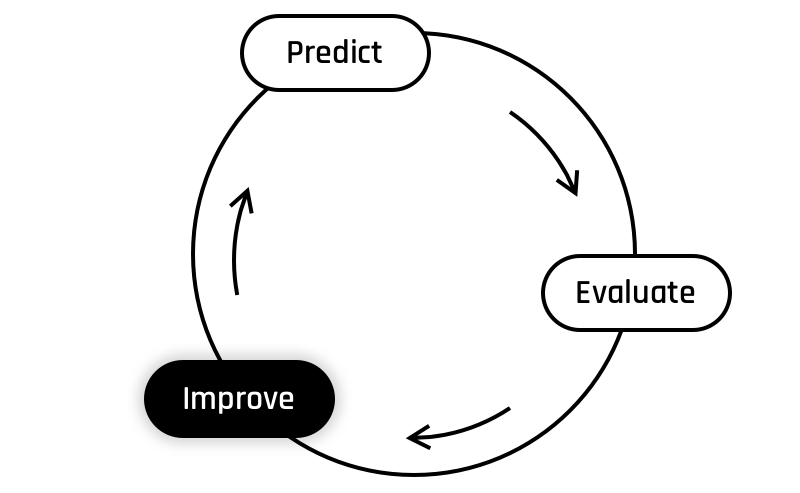
\includegraphics[scale=0.25]{assets/Improve.png}
    %\caption{The Learning Cycle: Improve}
\end{figure}
\noindent{To derive the gradient of the regularized loss function, $\nabla(J)$ 
you have to change a bit the formula of the unregularized gradient.}\\
\\
Given the fact that we are not penalizing $\theta_0$, the formula will remain 
the same as before for this parameter. For the other parameters ($\theta_1, \dots, \theta_n$),
 we must add the partial derivative of the regularization term: $\lambda \theta_j$.\\
\\
Therefore, we get:
$$
\nabla(J)_0 = \frac{1}{m}\sum_{i=1}^{m}(h_\theta(x^{(i)}) - y^{(i)})
$$
$$
\nabla(J)_j = \frac{1}{m}\left(\sum_{i=1}^{m}(h_\theta(x^{(i)}) - y^{(i)})x_j^{(i)} + \lambda \theta_j\right) \text{ for j = 1, ..., n}
$$
\\
Where:  
\begin{itemize}
    \item $\nabla(J)_j$ is the j$^\text{th}$ component of the gradient vector $\nabla(J)$
    \item $m$ is the number of training examples used
    \item $h_\theta(x^{(i)})$ is the model's prediction for the i$^\text{th}$ training example
    \item $x^{(i)}$ is the feature vector of the i$^\text{th}$ training example
    \item $y^{(i)}$ is the expected target value for the i$^\text{th}$ example
    \item $\lambda$ is a constant, the regularization hyperparameter
    \item $\theta_j$ is the j$^\text{th}$ parameter of the $\theta$ vector
\end{itemize}
\bigskip
Which can be vectorized as:
$$
\nabla(J) = \frac{1}{m} [X'^T(h_\theta(X) - y) + \lambda \theta']
$$  
\\
Where:  
\begin{itemize}
    \item $\nabla(J)$ is a vector of length $(n + 1)$, the gradient vector
    \item $m$ is the number of training examples used
    \item $X$ is a matrix of dimension $(m \times n)$, the design matrix
    \item $X'$ is a matrix of dimension $(m \times (n + 1))$, the design matrix onto 
    which a column of ones is added as a first column
    \item $y$ is a vector of length $m$, the vector of expected values
    \item $h_\theta(X)$ is a vector of length $m$, the vector of predicted values
    \item $\lambda$ is a constant
    \item $\theta$ is a vector of length $(n + 1)$, the parameter vector
    \item $\theta'$ is a vector of length $(n + 1)$, constructed using the following rules:
\end{itemize}

$$
\begin{matrix}
\theta'_0 & =  0 \\
\theta'_j & =  \theta_j & \text{ for } j = 1, \dots, n\\    
\end{matrix}
$$

% =============================================== %
\subsection*{Linear Gradient vs Logistic Gradient}
% ----------------------------------------------- %
As before, we draw your attention on the only difference between the linear regression's 
and the logistic regression's gradient equations: \textbf{the hypothesis function} $h_\theta(X)$.
\begin{itemize}
    \item In the linear regression: $h_\theta(X) = X'\theta$
    \item In the logistic regression: $h_\theta(X) = \text{sigmoid}(X'\theta)$
\end{itemize}

\newpage
\turnindir{ex04}
\exnumber{04}
\exfiles{reg\_linear\_grad.py}
\exforbidden{sklearn}
\makeheaderfilesforbidden


% ================================= %
\section*{Objective}
% --------------------------------- %
You must implement the following formulas as functions for the \textbf{linear regression hypothesis}\\

% ================================= %
\subsection*{Iterative}
% --------------------------------- %
$$
\nabla(J)_0 = \frac{1}{m}\sum_{i=1}^{m}(h_\theta(x^{(i)}) - y^{(i)})
$$
$$
\nabla(J)_j = \frac{1}{m}\left(\sum_{i=1}^{m}(h_\theta(x^{(i)}) - y^{(i)})x_j^{(i)} + \lambda \theta_j\right) \text{ for j = 1, ..., n}
$$
\\
Where:
\begin{itemize}
  \item $\nabla(J)_j$ is the j$^\text{th}$ component of $\nabla(J)$
  \item $\nabla(J)$ is a vector of dimension $(n + 1)$, the gradient vector
  \item $m$ is a constant, the number of training examples used
  \item $h_\theta(x^{(i)})$ is the model's prediction for the i$^\text{th}$ training example
  \item $x^{(i)}$ is the feature vector (of dimension $n$) of the i$^\text{th}$ training example,
   found in the i$^\text{th}$ row of the $X$ matrix
  \item $X$ is a matrix of dimensions $(m \times n)$, the design matrix
  \item $y^{(i)}$ is the i$^\text{th}$ component of the $y$ vector
  \item $y$ is a vector of dimension $m$, the vector of expected values
  \item $\lambda$ is a constant, the regularization hyperparameter
  \item $\theta_j$ is the j$^\text{th}$ parameter of the $\theta$ vector
  \item $\theta$ is a vector of dimension $(n + 1)$, the parameter vector
\end{itemize}

% ================================= %
\subsection*{Vectorized}
% --------------------------------- %
$$
\nabla(J) = \frac{1}{m} [X'^T(h_\theta(X) - y) + \lambda \theta']
$$  
\\
Where:
\begin{itemize}
  \item $\nabla(J)$ is a vector of dimension $(n + 1)$, the gradient vector
  \item $m$ is a constant, the number of training examples used
  \item $X$ is a matrix of dimensions $(m \times n)$, the design matrix
  \item $X'$ is a matrix of dimensions $(m \times (n + 1))$, the design matrix 
  onto which a column of ones is added as a first column
  \item $X'^T$ is the transpose of tha matrix, with dimensions $((n + 1) \times m)$
  \item $h_\theta(X)$ is a vector of dimension $m$, the vector of predicted values 
  \item $y$ is a vector of dimension $m$, the vector of expected values
  \item $\lambda$ is a constant, the regularization hyperparameter
  \item $\theta$ is a vector of dimension $(n + 1)$, the parameter vector
  \item $\theta'$ is a vector of dimension $(n + 1)$, constructed using the following rules: 
\end{itemize}

$$
\begin{matrix}
\theta'_0 & =  0 \\
\theta'_j & =  \theta_j & \text{ for } j = 1, \dots, n\\
\end{matrix}
$$
\newpage
% ================================= %
\section*{Instructions}
% --------------------------------- %
In the \texttt{reg\_linear\_grad.py} file, write the following functions 
as per the instructions given below:\\

\begin{minted}[bgcolor=darcula-back,formatcom=\color{lightgrey},fontsize=\scriptsize]{python}
def reg_linear_grad(y, x, theta, lambda_):
    """Computes the regularized linear gradient of three non-empty numpy.ndarray,
       with two for-loop. The three arrays must have compatible shapes.
    Args:
      y: has to be a numpy.ndarray, a vector of shape m * 1.
      x: has to be a numpy.ndarray, a matrix of dimesion m * n.
      theta: has to be a numpy.ndarray, a vector of shape (n + 1) * 1.
      lambda_: has to be a float.
    Return:
      A numpy.ndarray, a vector of shape (n + 1) * 1, containing the results of the formula for all j.
      None if y, x, or theta are empty numpy.ndarray.
      None if y, x or theta does not share compatibles shapes.
      None if y, x or theta or lambda_ is not of the expected type.
    Raises:
      This function should not raise any Exception.
    """
    ... Your code ...

def vec_reg_linear_grad(y, x, theta, lambda_):
    """Computes the regularized linear gradient of three non-empty numpy.ndarray,
       without any for-loop. The three arrays must have compatible shapes.
    Args:
      y: has to be a numpy.ndarray, a vector of shape m * 1.
      x: has to be a numpy.ndarray, a matrix of dimesion m * n.
      theta: has to be a numpy.ndarray, a vector of shape (n + 1) * 1.
      lambda_: has to be a float.
    Return:
      A numpy.ndarray, a vector of shape (n + 1) * 1, containing the results of the formula for all j.
      None if y, x, or theta are empty numpy.ndarray.
      None if y, x or theta does not share compatibles shapes.
      None if y, x or theta or lambda_ is not of the expected type.
    Raises:
      This function should not raise any Exception.
    """
    ... Your code ...
\end{minted}

\hint{
  this is a good use case for decorators...
}

% ================================= %
\section*{Examples}
% ================================= %
\begin{minted}[bgcolor=darcula-back,formatcom=\color{lightgrey},fontsize=\scriptsize]{python}
x = np.array([
		[ -6,  -7,  -9],
		[ 13,  -2,  14],
		[ -7,  14,  -1],
		[ -8,  -4,   6],
		[ -5,  -9,   6],
		[  1,  -5,  11],
		[  9, -11,   8]])
y = np.array([[2], [14], [-13], [5], [12], [4], [-19]])
theta = np.array([[7.01], [3], [10.5], [-6]])

# Example 1.1:
reg_linear_grad(y, x, theta, 1)
# Output:
array([[ -60.99      ],
		[-195.64714286],
		[ 863.46571429],
		[-644.52142857]])

# Example 1.2:
vec_reg_linear_grad(y, x, theta, 1)
# Output:
array([[ -60.99      ],
		[-195.64714286],
		[ 863.46571429],
		[-644.52142857]])

# Example 2.1:
reg_linear_grad(y, x, theta, 0.5)
# Output:
array([[ -60.99      ],
		[-195.86142857],
		[ 862.71571429],
		[-644.09285714]])

# Example 2.2:
vec_reg_linear_grad(y, x, theta, 0.5)
# Output:
array([[ -60.99      ],
		[-195.86142857],
		[ 862.71571429],
		[-644.09285714]])

# Example 3.1:
reg_linear_grad(y, x, theta, 0.0)
# Output:
array([[ -60.99      ],
		[-196.07571429],
		[ 861.96571429],
		[-643.66428571]])

# Example 3.2:
vec_reg_linear_grad(y, x, theta, 0.0)
# Output:
array([[ -60.99      ],
		[-196.07571429],
		[ 861.96571429],
		[-643.66428571]])
\end{minted}